\chapter{The Transit Monitoring in the South project}\label{chap:tramos}

The Transit Monitoring in the South (TraMoS) project started in 2008 aiming to perform photometric follow-up of transiting exoplanets using telescopes located in Chile.  Through photometric monitoring of transiting events, important information of the planetary system can be obtained, such as the planetary radius, inclination of the orbit, and, in combination with radial velocity data, the planetary mass, among others. Moreover, this kind of analysis allows the detection of variability in the transit's parameters (TPV), if several epochs of the transit event are obtained. The TraMoS project aims, on one hand, to refine the physical and orbital parameters of selected exoplanets systems through photometric follow-up and, on the other, to search for variations in those parameters that could suggest the presence of additional bodies in the system. 

To date, almost 400 transit events have been observed of 144 transiting exoplanets (see Figure \ref{tramos}). The bulk of the targets in the TraMoS project are hot Jupiters due to its short orbital period and large transit depth. Several facilities were used to perform the photometric follow-up such as the VLT of European Southern Observatory, the SMARTS 0.9 m and 1 m at Cerro Tololo Inter-American Observatory, the Danish 1.54 m at La Silla Observatory, SWOPE and Du Pont telescopes at Las Campanas Observatory and SOAR telescope at Cerro Pachón Observatory, among others. The diameter size of the used telescopes ranges from 0.6 meters to 8 meters. However, in the later stage of the TraMoS project, we built the team expertise using 1 meter-class telescope, for example in the Danish, SWOPE and SMARTS.

\begin{figure}[ht]
\centering
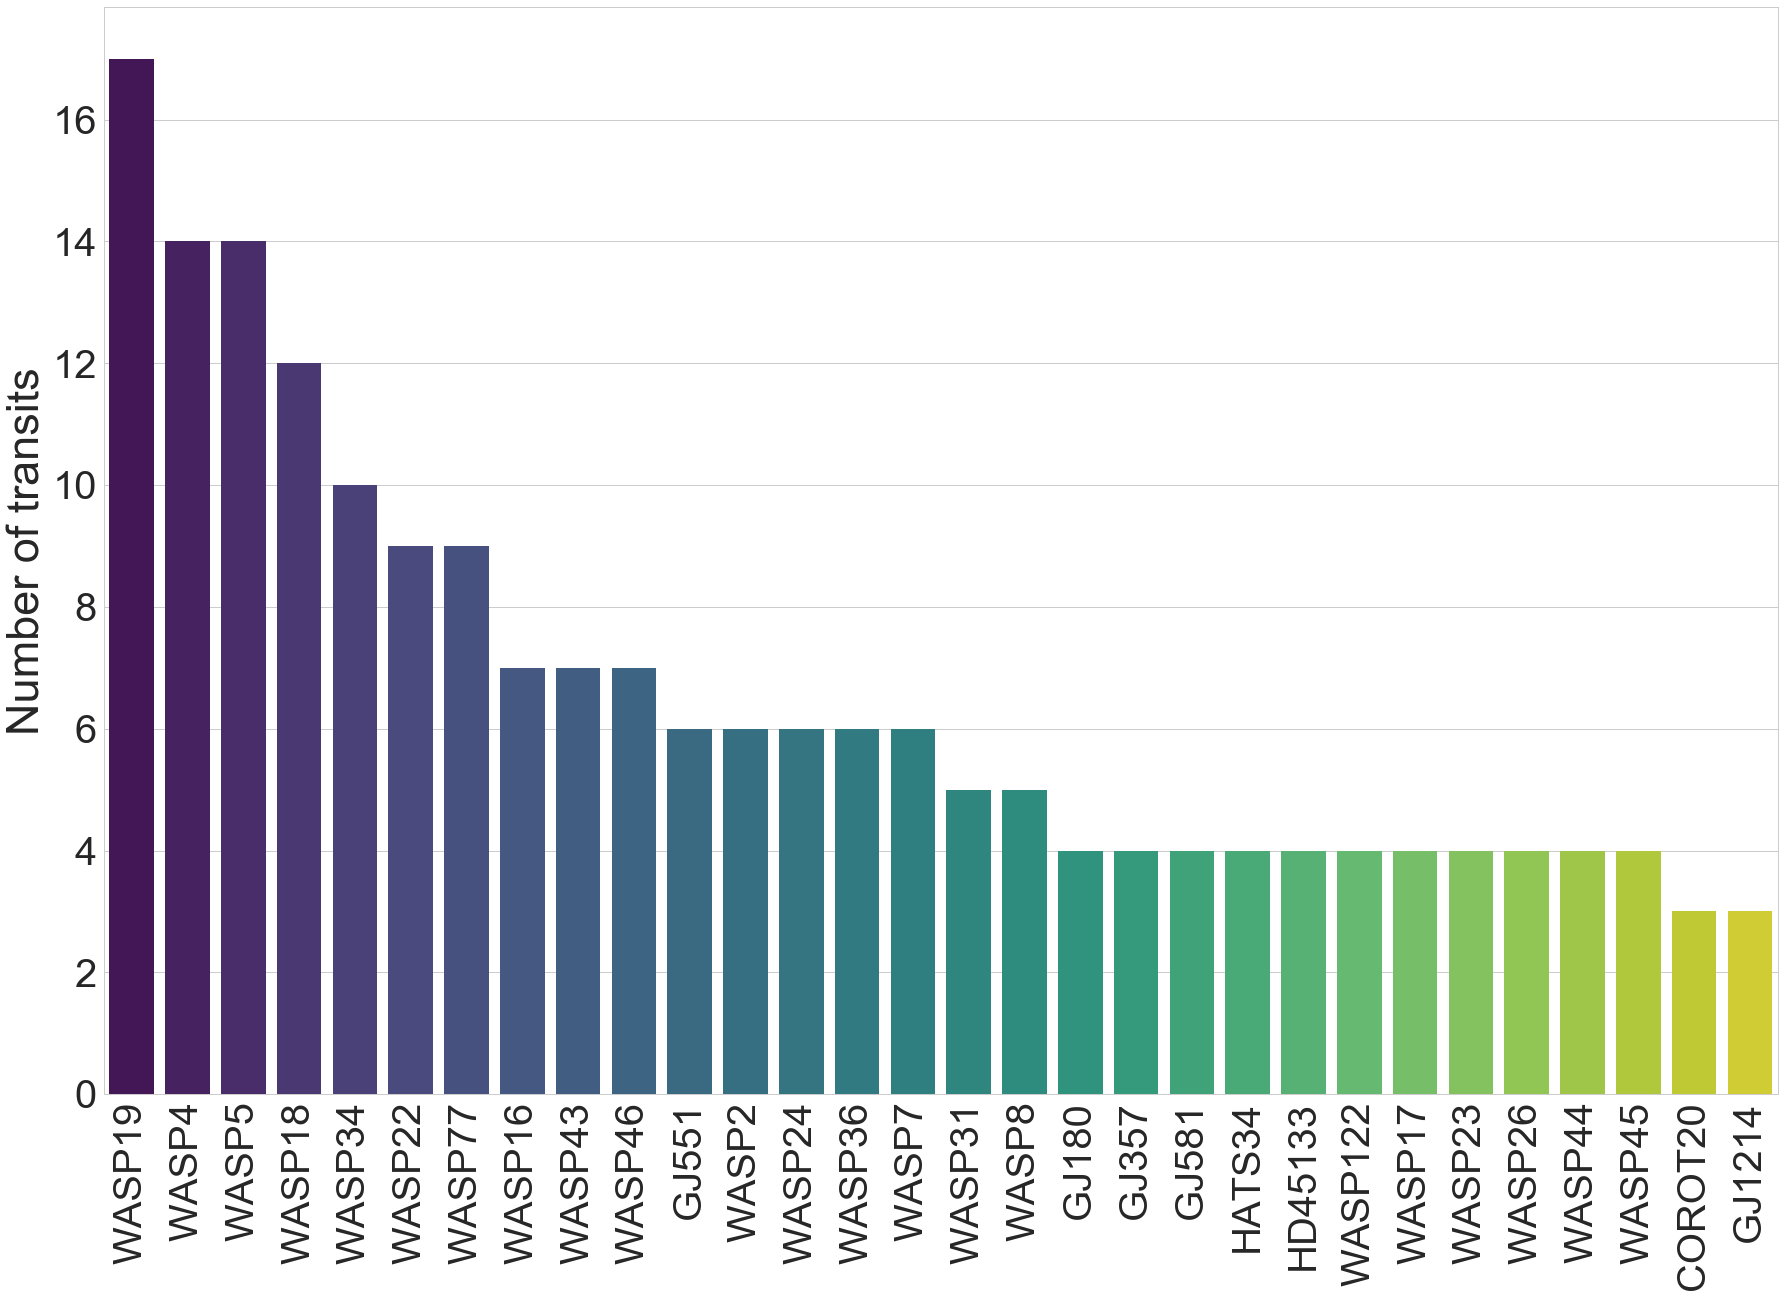
\includegraphics[width=0.9\columnwidth]{imagenes/tramos.png}
\caption{Histogram of the 30 transiting exoplanets with the largest amount of observations within the TraMoS project. The exoplanets WASP-4b and WASP5-b were presented in \cite{Hoyer2012} and \cite{Hoyer2013}, respectively. The results from the analysis of WASP-18b, WASP-19b and WASP77-Ab are in Cortés-Zuleta et al. 2019 (submitted, see Chapter \ref{chap:paper} for further details). In none of those systems a significant TPV signal was detected.}
\label{tramos}
\end{figure}


The first studies within the TraMoS project were conducted for Segio Hoyer's PhD dissertation (advisor: Patricio Rojo). Current results are summarized as: a possible orbital decay of WASP-43b \citep{Hoyer2016b} and OGLE-TR-113b \citep{Hoyer2016} was ruled out, and no significant TTV signal was detected in WASP-4b \citep{Hoyer2012} and WASP-5b \citep{Hoyer2013}.

In the following section \ref{lightcurve}, I describe the light curve produced from a transiting exoplanet --the principal target of the TraMoS project --  what information about the planet can be obtained from them and how these light curves can give us information about the architecture of this kind of systems. Then, in section \ref{ttv}, I detail on a specific type of phenomena of transiting exoplanets: the variation of the transit mid-time of its light curve (TTV).

\section{Transiting exoplanets' light curve\label{lightcurve}}

%\begin{figure}[ht]
%\centering
%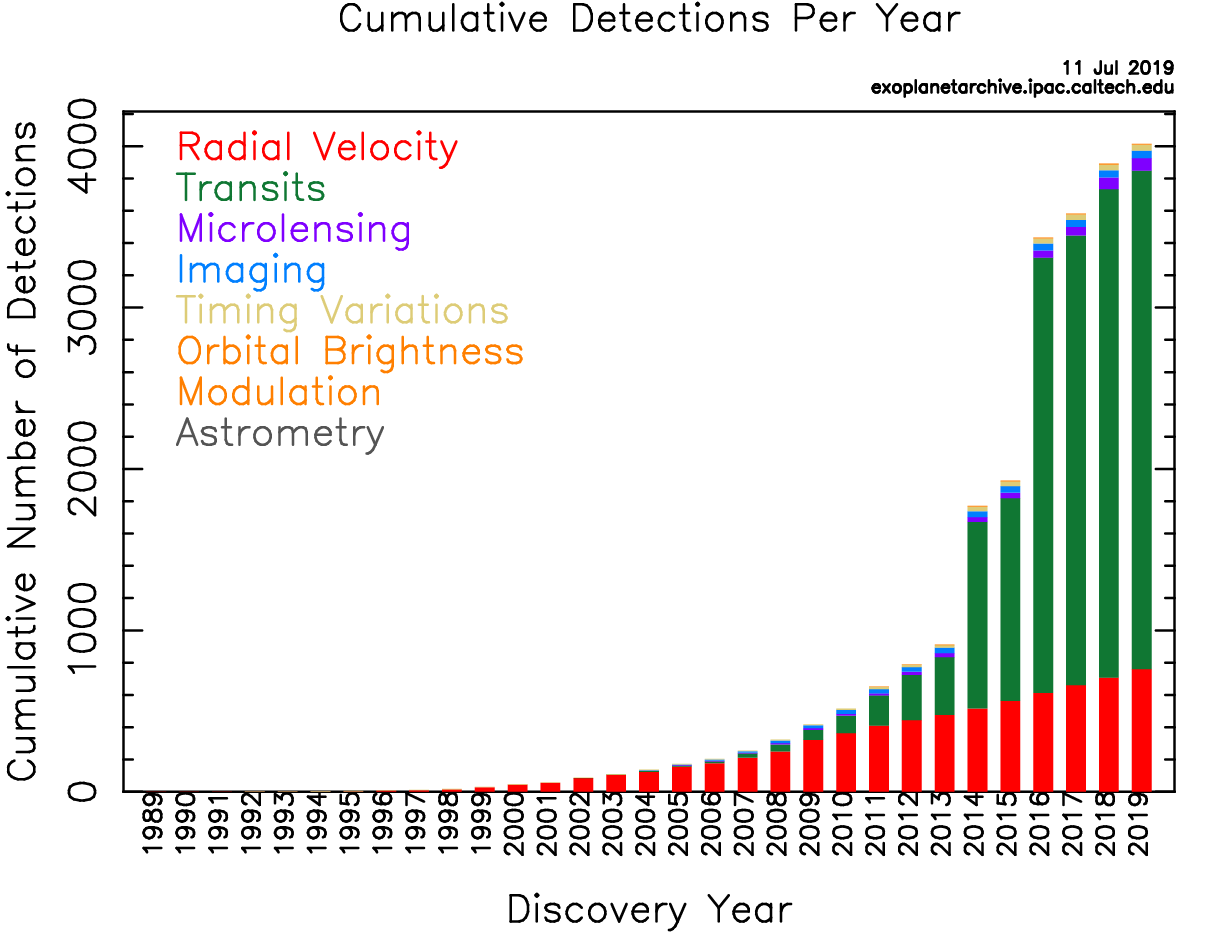
\includegraphics[width=0.7\columnwidth]{imagenes/exo_dischist_cumulative.png}
%\caption{Accumulative number of discovered exoplanets by year and their corresponding method of discovery. To date, the Transit technique, along with Radial Velocity, are the most successful methods to discovery exoplanets. Figure from the NASA Exoplanet Archive (\url{exoplanetarchive.ipac.caltech.edu})}
%\label{amount_exoplanet}
%\end{figure}

The light curve produced by a transit event provides important information about the planetary system. For example, it is the only way on which we can derive directly the proportion between the exoplanet and star radius. It can also give information about the impact parameter, and therefore, the inclination of the orbit. 

In Figure~\ref{transit} is shown the geometry of a transiting exoplanet. From geometric considerations the transit light curve and the parameters of the planetary system can be described with a few simple relations \cite{Seager2003,Winn2010}.  When the planet passes in front of its star produced a dimming in its flux called primary transit. The maximum drop during the transit event defines the transit depth $\Delta{F}$:

\begin{equation}
    \Delta{F} = \left(\frac{R_{p}}{R_{*}}\right)^2 
\end{equation}

Where $R_{p}$ and $R_{*}$ are the planet and star radius, respectively. The numbers 1, 2, 3 and 4 correspond to the contact times: $t_{1}$, $t_{2}$, $t_{3}$ and $t_{4}$ (see. Fig. \ref{transit}). The total duration of the transit is $t_{T} = t_{4}-t_{1}$ and the full duration is $t_{F}=t_{3}-t_{2}$. The total duration of the transit can be also described considering planetary parameters such as the period $P$, semi-major axis $a$ and orbital inclination $i$:

\begin{equation}
    t_{T} = \frac{PR_{*}}{\pi a} \sqrt{\left(1+\frac{R_{p}}{R_{*}}\right)^2-\left(\frac{a\cos i}{R_{*}}\right)}
\end{equation}

The impact parameter $b$, is the sky-projected distance between the center of the star and the planet at conjunction:

\begin{equation}
    b = \frac{a\cos{i}}{R_{*}}\left(\frac{1-e^2}{1+e\sin{\omega}}\right)
\label{impact_param}
\end{equation}

Where $\omega$ is the argument of pericenter. In the case of circular orbits, the eccentricity $e$ is zero, thus Eq.~\ref{impact_param} is simplified to:

\begin{equation}
    b = \frac{a\cos{i}}{R_{*}}
\label{impact_param_simple}
\end{equation}

\begin{figure}[ht]
\centering
\includegraphics[width=1.0\columnwidth]{imagenes/transit_architecture.pdf}
\caption{Geometry of a transiting exoplanet and the observed light curve. Based on the light curve itself it is possible to measure the transit depth $\Delta F$ and the orbit's inclination $i$. The numbers in circle indicate the four contact times: $t_{1}$, $t_{2}$, $t_{3}$ and $t_{4}$.  Figure from The Handbook of Exoplanets by M. Perryman.}
\label{transit}
\end{figure}

Depending on the orbital and physical parameters of the exoplanet, the shape of the observed light curve will vary. For example, Figure \ref{transit_examples} shows how the light curve reflects the configuration of the system. Hot Jupiters are the kind of planet that is relatively easier to detect since their planet-to-star radius ratio is larger, but a smaller planet orbiting a dwarf star could produce a similar ratio of the radius. On the other hand, exoplanets with smaller orbital inclinations will produce shallower drops in the flux, in comparison with planets in the same orbital-plane with the host star.     

\begin{figure}[h]
\centering
\includegraphics[width=0.8\columnwidth]{imagenes/transit_example.pdf}
\caption{Examples of transiting exoplanets and how their light curves differ between them thanks to the physical properties of the exoplanet.}
\label{transit_examples}
\end{figure}

When modeling the light curve's data, not only the physical parameters of the planet need to be taken into account, but the stars' too. The Limb Darkening effect of the star will change the shape of the observed light curve (during the time period $t3 - t2$ in Fig.~\ref{transit}), as what we are observing are photons coming from the star itself, especially when carrying-out observations with different filters. The effect of stellar limb-darkening describes the intensity variation across the disk of the star: the star appears brighter at the center and darker closer to the edge (stellar limb). The most general analytic formulae to model a light curve produced by a transiting exoplanet includes the Limb Darkening coefficients \citep{Mandel2002}, which can be quadratic or non-quadratic.

\section{Transit Timing Variations\label{ttv}}

Since the discovery of the first exoplanet, one of the principal questions that arose was: are they alone in their systems? The idea of multi-planetary systems is a consequence of our knowledge about the planetary system where we live in, and until today the Solar System has a larger number of orbiting planets. Besides the Solar System, Kepler-90 has the same number of confirmed exoplanets: eight. Statistically, around 20\% of the confirmed exoplanets are part of a multi-planetary system\footnote{Information obtained from the NASA Exoplanet Archive Database \url{https://exoplanetarchive.ipac.caltech.edu}}, but this number is theoretically larger. \cite{Fressin2013} computed the occurrence of exoplanets through numerical simulation with Kepler data, obtaining that around $52\%$ of the stars should have at least one planet within an 85 days orbit.

The Transit Timing Variations (TTV) technique was first proposed as a way to detect Earth-mass planets in multi-planetary systems due to gravitational interactions with a transiting exoplanet \citep{Holman2005,Agol2005}. However, as mention in Chapter \ref{chap:intro}, TTVs can be also used to measure tidal interactions between the planet and the star, such as orbital decays for instance, or to detect exomoons \citep{Kipping2009a,Kipping2009b}, among others phenomena in the star itself. 

For a given light curve of a transiting exoplanet (see Figure \ref{transit}), the transit mid-time $T_{c}$ (or central time of the transit) is computed as:

\begin{equation}
T_{c} = \frac{t_{4}+t_{1}}{2}
\end{equation}

A single (non-perturbed) transiting planet will stay in a Keplerian orbit around its host star, producing a transit time strictly periodic. Thus, the transit time $T_c$ follows a linear function in the transit epoch $E$: 

\begin{equation}
T_{c}(E) = T_{0} + E \cdot P
\label{linear_ephemeris} 
\end{equation}

Where $T_0$ is a reference transit time, $E$ is the number of epochs since $T_0$, and $P$ is the orbital period of the planet. The presence of a second (perturbing) planet produces transits no exactly periodic, hence Eq.~\ref{linear_ephemeris} will not be valid. As the transit times will be no longer a linear function,  the time between transits varies.  The variation in time produced by the perturber body depends on the mass and geometry of their orbits. The magnitude of this variation between successive transits of the transiting planet \citep{Holman2005}, assuming that the perturber body is in a inner orbit, $a_2 < a_1$, and follows a eccentric orbit with a periastron distance of $a_2(1-e_2)$, is:

\begin{equation}
\Delta t = \frac{45\pi}{16} \frac{M_2}{M_*} P_{1} \alpha^3_{e} (1-	\sqrt{2}\alpha_{e}^{3/2})^{-2}
\label{delta_t}
\end{equation}

Where $\alpha_e = a_1/(a_2(1-e_2))$ is the ratio of the semi-major axis of the planets, considering a nonzero eccentricity for the perturbing planet ($e_2 \neq 0$).The orbital period of transiting exoplanet is $P_1$, while the perturbing planet has a mass $M_2$, and orbital period $P_2$. The Eq. \ref{delta_t} obtains the best results, compared with numerical simulations, when $e_2>0.3$.

%When $e_2>0.3$, the relation \ref{delta_t} has the best performance with numerical simulations. 

Assuming that the orbital parameters of the known transiting exoplanet are already derived from its light curve, the orbital parameters and mass of the hypothetical perturber can be estimated numerically \citep{Nesvorny2008,Nesvorny2009}, even if the second planet does not transit the star. 

The TTV method is an efficient tool to search for additional unseen companions since, to employ this technique, only photometry of the transiting exoplanet during transit events is required. Moreover, this technique enhances its sensitivity when the two bodies in the system are close to Mean Motion Resonances (MMR) \citep{Agol2005,Steffen2005,Agol2007} (see Figure~\ref{rms_ttv_amplitude}) . 

\begin{figure}[ht]
\centering
\includegraphics[width=1.0\columnwidth]{imagenes/jupiter_ttv.pdf}
\caption{Example of a system with a transiting exoplanet of $1~M_{J}$ in a 10-day orbit and an Earth-mass perturber planet. The top panel is an Observed minus Computed diagram showing the measured TTV of the Jupiter-mass planet when the perturber has a period of 16.11 days, not in Mean Motion Resonance with the transiting planet. The panel at the bottom shows the TTV of the transiting planet when both are near an interior 2:1 resonance. In this case, the small planet has a period of 19.7 days. The amplification of the TTV signal is by an order of magnitude. Figure generated with the Python package: \texttt{ttv2fast2furious}.}
\label{rms_ttv_amplitude}
\end{figure}

\cite{Holman2010} presented the first multi-planetary system confirmed using the TTV method: two planets orbiting Kepler-9, a Sun-like star. These two Saturn-size planets are in near 2:1 orbital resonance with periods of 38.9 and 19.2 days. To model the dynamical interaction of the system, only 9 transits of Kepler-9b and 6 from Kepler-9c were required. This confirmed the effectiveness of the TTV method to characterize planetary systems with a scarce number of transits.

Since the discovery of \cite{Holman2010}, around 20 exoplanets have been discovered and characterized thanks to the measurement of variations on their transit times and the following proper dynamical modeling of the system. Most of them are Kepler systems because of its high duty-cycle, on which it provided years on transits data. Kepler stopped working on 2018, but the Transit Exoplanet Satellite Survey (TESS) is currently delivering its first results with new planetary systems showing TTVs.  For example, two exoplanets -- possibly one Jupiter and a sub-Saturn like -- were recently discovered by \cite{Dawson2019} orbiting TOI-216, in near 2:1 resonance. 

To date, only two hot Jupiters have been found to show TTV signals due to the presence of additional companions on their systems: WASP-47b \citep{Becker2015} and Kepler-730b \citep{Canas2019}, even though the TTVs was proposed as a technique to search for additional companions of gas giants. The lack of observed companions in hot Jupiter systems could provide crucial information about planetary formation processes. Through the TTV method not only the transiting exoplanet is being studied but the whole planetary system. 

\cite{Steffen2012b} analyzed Kepler data to constrain the occurrence rate of companions in hot Jupiter system. In a sample of 63 hot Jupiter candidates, none of them show evidence of possible companions in their system. When comparing with other types of exoplanets, 30\% of hot Neptune candidates may have companions and 10\% of warm Jupiter candidates. This could suggest that hot Jupiter may have different formation processes on which smaller companions are not allowed in their system: probably they are ejected through planet-planet scatter during migration. TTV studies could provide important clues about formation processes and dynamical evolution, and their mass and period dependency. 